\documentclass{article}
\usepackage[top=1in, bottom=1in, left=1in, right=1in]{geometry}
\usepackage[utf8]{inputenc}
\usepackage[T1]{fontenc}
\usepackage{amsmath}
\usepackage{amssymb}
\usepackage{lmodern}
\usepackage{bm}
\usepackage{scrextend}
%\usepackage{showframe}
\usepackage{calc}
\usepackage{changepage}
\usepackage{mdframed}
\usepackage{dsfont}
\usepackage{enumitem}
\usepackage{pbox}
\usepackage{setspace}
\usepackage{stmaryrd}
\usepackage{setspace}
\usepackage[table]{xcolor}
\usepackage{multicol}
\usepackage{mathtools}
\usepackage{hanging}
\usepackage{longtable}
\usepackage{aligned-overset}
\usepackage{ntheorem}
\usepackage{mdframed}
\usepackage[theorems,breakable]{tcolorbox}

\usepackage[,sorting=none,backend=biber,style=numeric,citestyle=numeric]{biblatex}

\allowdisplaybreaks
\hbadness=10000
\makeatletter
\renewcommand*\env@matrix[1][*\c@MaxMatrixCols c]{%
  \hskip -\arraycolsep
  \let\@ifnextchar\new@ifnextchar
  \array{#1}}

\newcommand{\mathleft}{\@fleqntrue\@mathmargin10pt}
\newcommand{\mathcenter}{\@fleqnfalse}
\makeatother

\newcommand*{\QED}{\hfill\ensuremath{\square}} 
\newcommand{\R}{\mathbb{R}}
\newcommand{\N}{\mathbb{N}}
\newcommand{\Z}{\mathbb{Z}}
\newcommand{\Q}{\mathbb{Q}}
\newcommand{\p}{\mathcal{P}}
\newcommand{\K}{\mathbb{K}}
\newcommand{\C}{\mathbb{C}}
\newcommand{\la}{\langle}
\newcommand{\ra}{\rangle}


\newcommand{\bol}[1]{\mathbf{#1}}


\newlength{\hangwidth}
\newcommand{\newhang}[1]{\settowidth{\hangwidth}{#1}\par\hangpara{\hangwidth}{1}#1}

\newcommand{\norm}[1]{\lVert #1 \rVert}

\def\Abstand{1cm}

\newtcbtheorem{lemma}{Lemma}{%
        theorem name,%
        colframe=gray,%
        fonttitle=\bfseries,
        boxsep=5pt,
        left=5pt, right=5pt, top=5pt, bottom=5pt
    }{lem}

\newtcbtheorem{theorem}{Theorem}{
        theorem name,%
        colframe=gray,%
        fonttitle=\bfseries,
        boxsep=5pt,
        left=5pt, right=5pt, top=5pt, bottom=5pt
    }{thm}

\newtcbtheorem{definition}{Definition}{
      theorem name,%
      colframe=gray,%
      fonttitle=\bfseries,
      boxsep=5pt,
      left=5pt, right=5pt, top=5pt, bottom=5pt
  }{def}

\title{Compositional Generative Modeling}
\author{ }
\date{}
\addbibresource{lib.bib} % BibLaTeX bibliography file


\begin{document}


\maketitle

\newlength\breite
\setlength\breite{\linewidth-4pt}
\setlength\fboxsep{0pt}
\setlength\fboxrule{0.25pt}
\setlength{\abovedisplayskip}{3mm} %Abstand OBEN zw. Text und Formel
\setlength{\belowdisplayskip}{3mm} %Abstand OBEN zw. Text und Formel
\setlength\itemsep{0pt}
\setlength\parindent{0pt}


\mathleft

\section*{Introduction}

Generative Models have had tremendous success in recent years, to train them to generalize in complex and changing environments is challenging, which is why compositionality is a desirable property. 

What we want, is for two learned generative models(i.e. Diffusion, Flow Matching etc.), represented by their learned densities $p_{D_1}$ and $p_{D_2}$ on some datasets $D_1$ and $D_2$ to be able to sample from $$p_{comp} \propto p_{D_1} \cdot p_{D_2}$$ where the normalization constant $Z$ given by:
\[
Z = \int_{\R^d} p_{D_1}(x) \cdot p_{D_2}(x) \, dx.
\]
is not tractable in practice (if we assume data in $\R^d$ which is not too restrictive for now). To do this, multiple naive and more involved ideas exist, which we will try to explore in this document, focussing on toy datasets. \\

Intuitively, in the case seems clear at first glance in the case of diffusion models where we have trained score $\nabla \log p^i_{t}$ with $p_1 \approx p_{D_1}$ for $i \in \{1,2,...,n\}$ (in general, for now we consider $n = 2$) and $t \in [0,1]$ then, we have $$\nabla \log (p_{D_1} \cdot p_{D_2}) = \nabla \log p_{D_1} + \nabla \log  p_{D_2} \approx \nabla \log p^2_{1} + \nabla \log  p^1_{1}$$ 

which seems to solve the issue. However, as pointed out in \cite{reduce} problems arise (we actually got aware of this paper after conducting similar experiments to theirs). Namely, when sampling we utilize the score evolving through time, for the true product $p^t_{comp}$ this can be written as $$\nabla \log p^t_{comp} (x_t) = \nabla \log \left( \int_{\R^d} \cdot p(x_t \mid x) p_{D_1}(x) p_{D_2}(x)dx \right)$$ 
which in general will not equal to $$\nabla \log \left( \int_{\R^d} \cdot p(x_t \mid x) p_{D_2}(x)dx \right) + \nabla \log \left( \int_{\R^d} \cdot p(x_t \mid x) p_{D_1}(x)dx \right)$$

Thus, the above only really works well for independent $D_1$ and $D_2$ which is rarely the case. 


\newpage 
Imagine we have the following diffusion models trained on the following distributions. 

\begin{center}
\begin{minipage}{0.4\textwidth}
  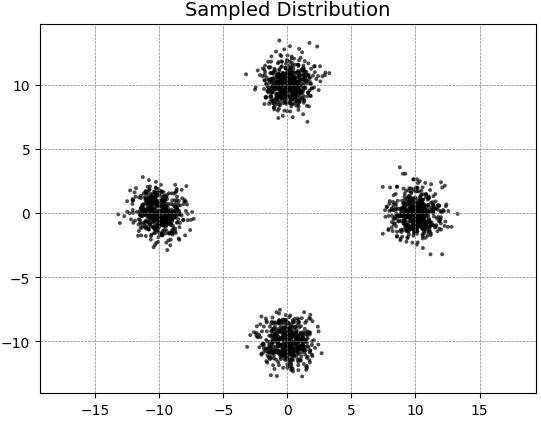
\includegraphics[width=\linewidth]{images_guidance1/GaussianMixtureForAddedScores.png}
  \centering\small $p_{D_1}$
\end{minipage}
\hfill
\begin{minipage}{0.4\textwidth}
  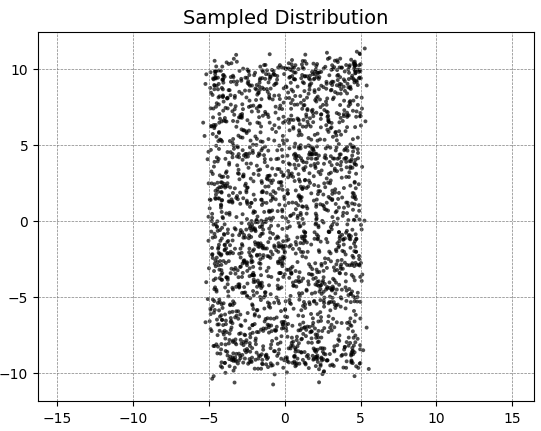
\includegraphics[width=\linewidth]{images_guidance1/RectangleforGaussianMixtureaddedScores.png}
  \centering\small $p_{D_2}$
\end{minipage}
\hfill
\end{center}


Then, just adding their scores gives the following, which is of course not the true product.


\begin{center}
  \centering
\begin{minipage}{0.7\textwidth}
  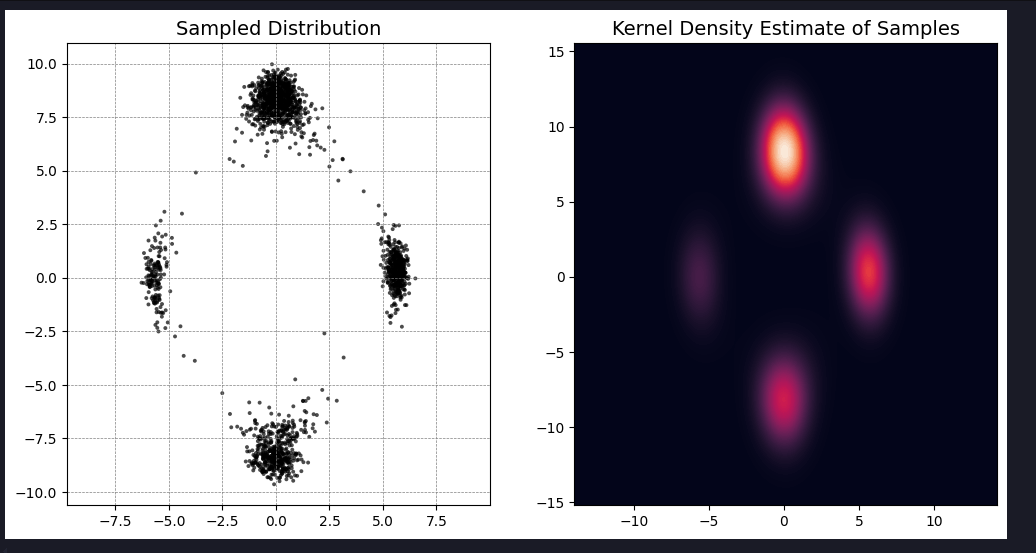
\includegraphics[width=\linewidth]{images_guidance1/addingscoresGaussianMixtureandRectangle.png}
  \centering\small $p_{comp}$ ?
\end{minipage}

\end{center}

However, in the case where we have simpler distributions with better behaved overlap, it works a bit better (why?). (here $D_2$ is the same pair of rectangles just rotated 90 degrees)

\begin{center}
  \begin{minipage}{0.4\textwidth}
    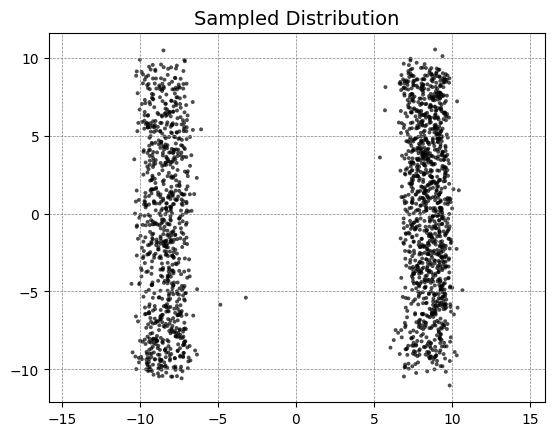
\includegraphics[width=\linewidth]{images_guidance1/model1foraddedscores.png}
    \centering\small $p_{D_1}$
  \end{minipage}
  \hfill
  \begin{minipage}{0.4\textwidth}
    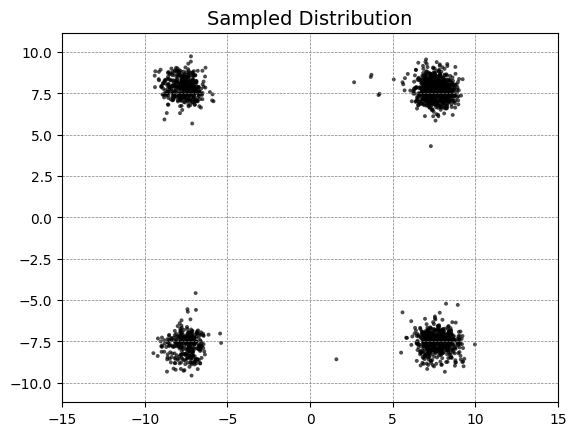
\includegraphics[width=\linewidth]{images_guidance1/addedscores1.png}
    \centering\small $p_{comp}$
  \end{minipage}
  \hfill
  \end{center}


\newpage
Even if the supper of the product is not 'symmetric', it still somewhat works, although not the entire support is covered. 
Here $D_2$ is the distribution of the two rectangles above. 
\begin{center}
  \begin{minipage}{0.4\textwidth}
    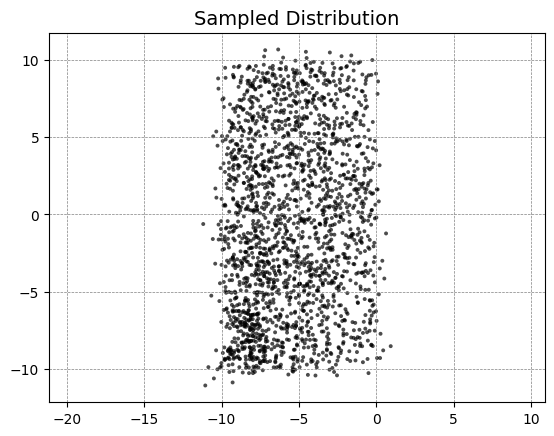
\includegraphics[width=\linewidth]{images_guidance1/Rectangleforaddedscores2.png}
    \centering\small $p_{D_1}$
  \end{minipage}
  \hfill
  \begin{minipage}{0.4\textwidth}
    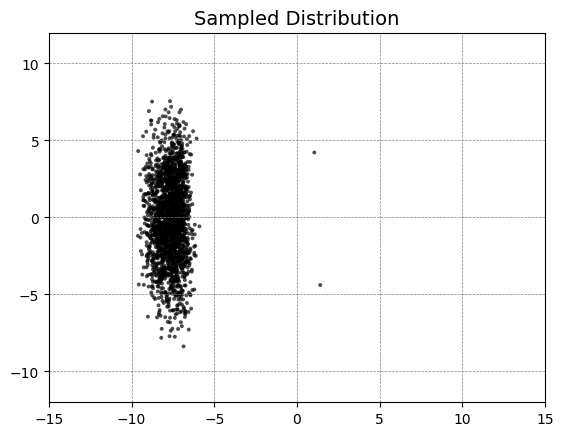
\includegraphics[width=\linewidth]{images_guidance1/addedscores2.png}
    \centering\small $p_{comp}$
  \end{minipage}
  \hfill
  \end{center}


Other approached for this problem have been widely explored, in \cite{liu2023compositionalvisualgenerationcomposable} they, instead of working with independently trained models work with Diffusion guidance and certain 
pre-specified concepts $(c_1,...,c_n)$ they which to 'compose' i.e. they want to have both $c_1$ and $c_2$ present in an image, or they want $c_1$ NOT in the image etc. This was also discussed in \cite{reduce} and \cite{bradley2025mechanismsprojectivecompositiondiffusion}. \\

They do this, by utilizing diffusion guidance and utilizing an 'unconditional' Model as the baseline, which in their case is just the union since they are inspired by guidance, in \cite{bradley2025mechanismsprojectivecompositiondiffusion} and \cite{reduce} they discuss why this approach could fail. 

After first testing, we, for the simple four overlapping rectangles, see that (up to numerical errors?) the guidance works for getting the product of two concepts. 
 
\begin{center}
  \centering
\begin{minipage}{0.7\textwidth}
  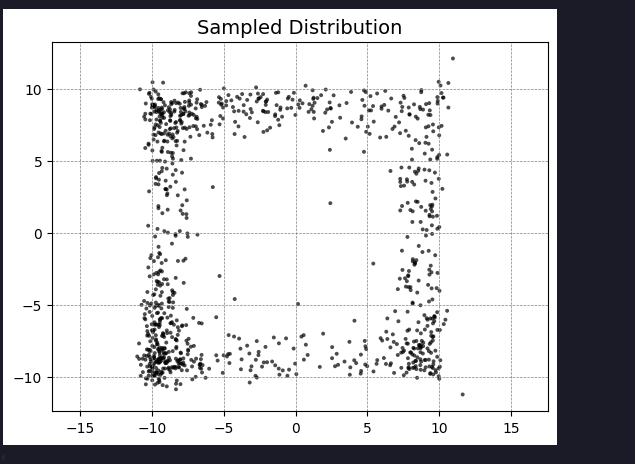
\includegraphics[width=\linewidth]{images_guidance1/unconditionalguidance.png}
  \centering\small Unconditional 
\end{minipage}

\end{center}

Now, when conditioning on only one rectangle, or two rectangles at the same time, we get. 

\begin{center}
  \begin{minipage}{0.4\textwidth}
    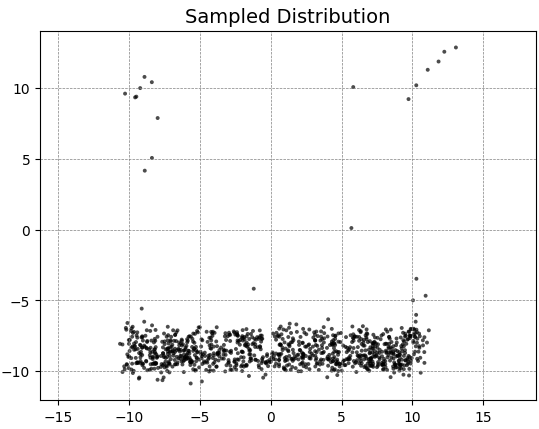
\includegraphics[width=\linewidth]{images_guidance1/conditionedononerectangle.png}
    \centering\small $p_{D_1}$
  \end{minipage}
  \hfill
  \begin{minipage}{0.4\textwidth}
    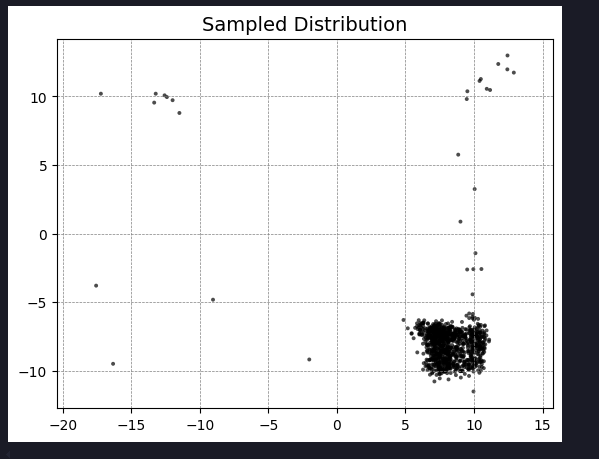
\includegraphics[width=\linewidth]{images_guidance1/productofconditioningontworectangles.png}
    \centering\small $p_{comp}$
  \end{minipage}
  \hfill
  \end{center}

But, even if not working perfectly, we can see that on these toy datasets, the guidance approach somewhat works in the above setting of rectangle and Mixture of Gaussians. 

\begin{center}
  \centering
\begin{minipage}{0.7\textwidth}
  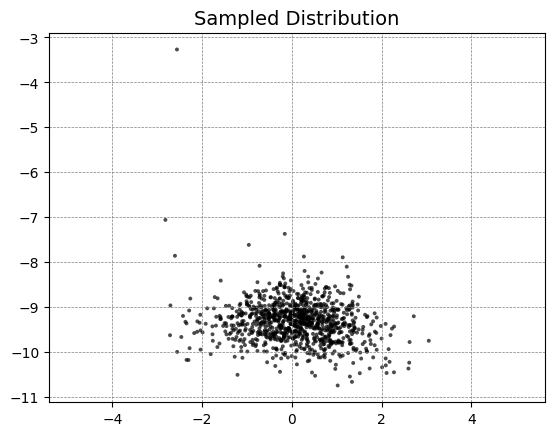
\includegraphics[width=\linewidth]{images_guidance1/productofsquareandonemode.png}
  \centering\small Guidance on one Mode and the Rectangle
\end{minipage}

\end{center}


metrics: KL, Wasserstein, \textbf{https://en.wikipedia.org/wiki/Jensen%E2%80%93Shannon_divergence

\printbibliography

\end{document}